\documentclass[12pt, letterpaper]{article}  % it must be at least 11 pt or more if you like (here we used 12 for clarity of the demo), and change article with report
\usepackage[letterpaper, top=3.71cm, bottom=3.20cm, left=2.86cm, right=2.86cm]{geometry}
%top = 2.44 (header in doc) + 1.27
% bottom 1.42 (footer in doc) + 1.78
\usepackage[utf8]{inputenc}
\usepackage{natbib}
\usepackage{graphicx}
\usepackage{color}

\title{\vspace{-2cm}\textbf{Title}}
\author{\small{Authors (\textit{Name Surname}).} \\ % put your full name here
        \small{Master Degree (curriculum). \underline{Emails}.} \\  % put your Master Degree (and curriculum) here
        \small{ML course (exam code), Academic Year: \dots} \\
        \small{Date: xx/yy/xyzz} \\
        \small{Type of project: \textbf{A/B/C} \textit{(see below)}}
}

\renewcommand\refname{} %remove this line to automatically show the bibliography header

\begin{document}
\nocite{*}  % comment this line to list only the articles you really cite
\date{}
\maketitle

\noindent\fbox{%
    \parbox{\textwidth}{%
        Notes to you:
        \begin{itemize}
            \setlength\itemsep{0em}
            \item File name: Use the surnames of the group components
            \item Language: English (Italian as a special case, spelling and clarity are essential)
            \item Use word if you like, but  latex is better. Anyway, send a PDF file
            \item \textbf{Font 11} at least! (here font 12 for clarity) $\leftarrow$ Mandatory (else we will reject)
            \item Type of project : can be A/B/(C)
            \begin{itemize}
                \setlength\itemsep{0em}
                \item[$\circ$] \textbf{A} (new NN simulator with your code, in that case specify the programming  language) or specify \textbf{A with CM}
                \item[$\circ$] \textbf{B} (comparing existing simulators, specify which ones)
                \item[$\circ$] \textbf{C} (rare and ad hoc case, refer our agreement,email and date)
            \end{itemize}
            \item Pages: up to \textbf{8} [2 students case], up to \textbf{10} pages for 3 students project [\underline{[standard case}]: use appendix for large or other tables or plots (if needed); \underline{the pages out of the limit will be not read nor evaluated}!!! $\leftarrow$ Important
            \item See instructions in the slides of the lecture for the project description!
        \end{itemize}
    }%
} 
\begin{abstract}
Insert here few rows (up to 5) summarizing the developed project (\underline{used model} \underline{for the cup}, validation technique, novelties if any) \dots
\end{abstract}

\section{Introduction}
Describe/define \textit{your aim and the essential background} (\underline{in short}):
\begin{itemize}
    \setlength\itemsep{0em}
    \item[$\circ$] Define your aims: To explore/improve what? What are you going to show?
    \item[$\circ$] Describe (just \underline{define}) the used models, the used algorithms  etc. 
    \item[$\circ$] Describe your assumptions (if any significant).
\end{itemize} 

\section{Method (be schematic!)}
\underline{Briefly} (short part) describe \textit{what you developed and how}:
\begin{itemize}
    \setlength\itemsep{0em}
    \item[-] The code (for type A implementation) or the used simulator(s) (for type B). 
        \begin{itemize}
            \setlength\itemsep{0em}
            \item[$\circ$] The used tools/libraries (if any) 
            \item[$\circ$] Software overview and the software design choices (if interesting)
            \item[$\circ$] Implementation choices (a summary): e.g. architecture/s (and numb. of layers), type of activation function/s, type of training algorithm/s, batch/on-line/mb, initialization schema/s, regularization schema/s, stop condition/s.
            \item[$\circ$] The novelties (if any) but not the standard approaches (\underline{\textit{do not}} describe the algorithms/models we already described in the lectures). Use references for the source of information. 
        \end{itemize}
        \item[-] Preprocessing procedure (if any) [details may be postponed to Section \ref{sec:experiments}]
        \item[-] \underline{Validation schema} (model selection and evaluation schema) for the Experimental part: report data splitting  TR/VL/TS (\% data for each set and/or the K values of the K-fold CV) [details may be postponed to Section \ref{sec:experiments}]
        \item[-] Type of preliminary trials pursued (often summarized by text) [details may be postponed to Section \ref{sec:experiments}]
\end{itemize}


\noindent \\ Each figure/table should be referenced as in the following, see Fig \ref{fig:myfigure}. 
Do not use figure/table without a number. Do not write “see the next figure” (which one?).
Tables and plots have always a caption. All of the Figures and Tables should be cited in order, including those in the Appendix. (which should be cited as, for example, Fig. A.1, and Table A.1).  

\begin{figure}[h]
\centering
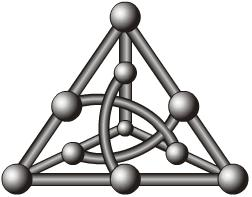
\includegraphics[width=0.3\textwidth]{figure.jpg}
\caption{Do \textit{not} insert a picture of your network (unless it is innovative).}
\label{fig:myfigure}
\end{figure}

\newpage
\section{Experiments}
\label{sec:experiments}
\textit{What you have found}: The results should be the \underline{larger part} of the report.

\vspace{-0.3cm}\subsection{Monk Results (Schematic!)}
In this subsection report only plots and tables, comment only if needed and very short. \\
\textcolor{red}{[*] Lack of results in this part invalidates the report.  Both for A and B prj} (and for all the considered models of prj B). \\
Please report:
\vspace{-0.4cm}\begin{itemize}
    \setlength\itemsep{-0.5em}
    \item[-] Performance (see Table \ref{tab:monk-table}) and learning curves (MSE and accuracy plots for the 3 MONK’s tasks, see Fig. 2 as an example filled with the plot for the MONK2)
    \item[-] Used hyper-parameters
\end{itemize}
\vspace{-0.5cm}\begin{table}[h]
\centering
\small
\begin{tabular}{|l|l|l|l|}
\hline
\textbf{Task} & \textbf{\#Units, eta, lambda, ..} & \textbf{MSE (TR/TS)} & \textbf{Accuracy (TR/TS)(\%)\textsuperscript{\textcolor{red}{i}}} \\ \hline
MONK1         &                                   &                      &                                \\ \hline
MONK2         &                                   &                      &                                \\ \hline
MONK3         &                                   &                      &                                \\ \hline
MONK3+reg. &                                   &                      &                                \\ \hline
\end{tabular}
\caption{Average prediction results obtained for the MONK’s tasks.}
\label{tab:monk-table}
\end{table}

\vspace{-0.5cm}
\begin{figure}[h!]
\centering
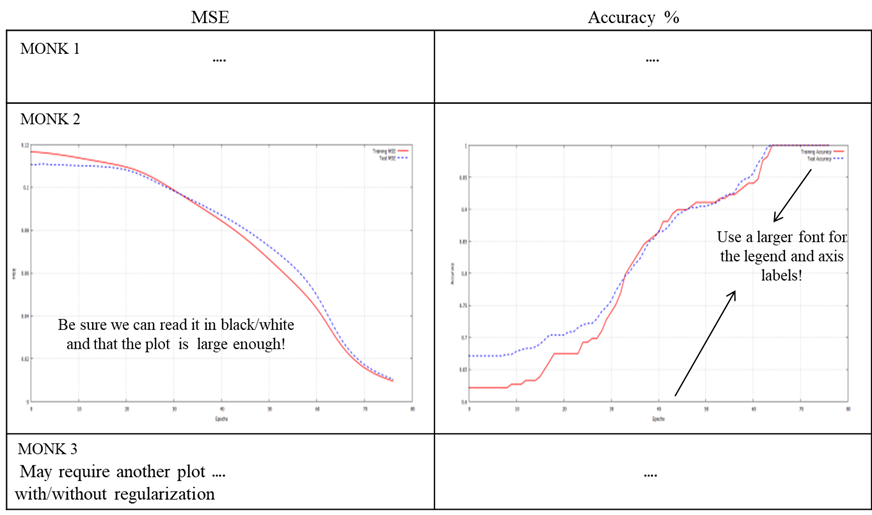
\includegraphics[width=\textwidth]{monkplot.png}
\caption{Plot\textsuperscript{\textcolor{red}{\textbf{ii}}} of the MSE and accuracy for the 3 MONK’s benchmarks. [Be sure it will be easy to read them in Black\&White (after print) with enough large font]}
\label{fig:monkplot}
\end{figure}

\newpage

\subsection{\underline{Cup Results} (Detailed!)}
\underline{\textbf{\textit{Always include:}}}
\begin{enumerate}
    \setlength\itemsep{-0.2em}
    \item \underline{Details of the Validation schema} (model selection and assessment): Splitting \\ TR/VL/(internal)TS (\% of data for each set and/or the K values of the K-fold CV)  \textcolor{red}{[*]}
    \item Screening phase: Type of preliminary trials pursued (often summarized by text) 
    \item Schema and \underline{range} of explored hyper-parameters (values used for the grid search, possibly a table) \textcolor{red}{[*]}
    \item Grid search: \underline{TABLES of results} TR/VL/(TS)\textsuperscript{\textbf{\textcolor{red}{iii}}} with MEE \textcolor{red}{[*]}. At least the most performant cases. Tables/Plots can be used also to show some relevant trends for specific hyper-parameters changes (if you think it is significant) 
    \item Provide an estimation of the (training) computing time (and of your HW resources)
    \item Repeat and compare if you are comparing different models/algorithms/approaches (or different variants of the approach that you think are significant). 
    \item \textbf{\textit{Define how you selected the}} \underline{FINAL model} used on the blind test set \textcolor{red}{[*]}. \underline{Which is it among the candidates and why?} Also write the  hyper-param. of the final model \textcolor{red}{[*]}.
    \item \textbf{\textit{Report}} for the \underline{FINAL model} used on the blind test set the \underline{TABLE with MEE} for \underline{TR (training)}, \underline{VL (validation)} and \underline{TS (internal TS)}\textsuperscript{\textbf{\textcolor{red}{iv}}} \underline{in the original scale} \textcolor{red}{[*]}\textcolor{red}{[*]}. Note again  that you must have an internal  test evaluation (see the note IV above)
    \item Plot the \underline{learning curve} TR/(VL)\textsuperscript{\textbf{\textcolor{red}{v}}}/TS for the  FINAL model \textcolor{red}{[*]} (it is unique) 
    \item \textbf{Discussion} (what you found more significant in your experiments, it is a relevant part!)
\end{enumerate}
\textcolor{red}{[*] = Lack of results in this part invalidates the report. Both for A and B prj.} \\

\noindent\textit{\textbf{Further explanations and notes:}}

{\footnotesize
A good experimental report lists observed facts \textit{supported by experimental evidence}:
\begin{itemize}
    \setlength\itemsep{-0.25em}
    \item[$\circ$] Report of used  setting (\textbf{\textit{replicability}}), and of the procedure for model selection and validation/assessment
    \item[$\circ$] Report accurate results in numerical and graphical form (clear tables/plots with measures of training, validation and test errors)
    \item[$\circ$] Make a selection of the evidences that you think are important but for those  show with graphs / tables etc, e.g. by plots varying the hyperparameters values
    \item[$\circ$] Make critical remarks (+/-) on the effect of your choices (and, if necessary, their agreement with the theory of ML or report and discuss unusual evidences)
    \item[$\circ$] Note that the relative position between the different cases is interesting (not the absolute performance)
    \item[$\circ$] Learning curve to show the TR, Val/Test error with the progress of training: Curve with LMS (loss used for training) and measure of final error curve (e.g. accuracy for classification) can be different
 
\end{itemize}

   }      %% end of footnote size
        
\section{Conclusion}
\textit{What you have drawn} and also:

BLIND TEST RESULTS: name of the result files  and your nickname

\section*{Acknowledgments}
If any. \\ \\

\noindent\textit{We agree to the disclosure and publication of our names, and of the results with preliminary and final ranking.}

\section*{References}
From where you are taking information, where a reader can find details, credits, sources \dots See any paper bibliography to take examples. The items here should be numbered and the number should be used in the text. \textbf{Double check the bibliography}!!! \\ \\
In particular, always include (with a uniform style): \\

Authors, Title, Journal/Proceedings/Editor, Volume, Pages, Year (URL if needed) \\ \\
E.g. see the following references: 
\bibliographystyle{plain}
\vspace{-1cm}\bibliography{mybib}

\newpage

\section*{Appendix A}
If needed, insert here (only) \underline{TABLES, GRAPHS, \textbf{PLOTS}} that are \textbf{not} essential in the main sections, or that are too large. 
Take care: The report can be read without reading the appendix. 
These parts may be out of the maximum 8/10 pages, without a specific limit (but should be reasonable!). \\ \\ 

\noindent\rule{6cm}{0.4pt} \\
\noindent \textsuperscript{\textbf{i}} Please see FAQs in the PRJ lecture: report the \underline{mean} result over the different initialization, not just the best result. Moreover, remember that the  MSE does not  include the penalty term. \\ \\
\textsuperscript{\textbf{ii}} General note on plots in the report: to be comparable,  use  \underline{a point for} \underline{each epoch} (defined as the total number of training data): if you are using on-line or mini-batch provide the mean over an epoch for each point in the plot.
\textsuperscript{\textbf{iii}}  The internal test set (see the note IV) results can be or can be not present during the grid search according to your decisions on the  data splitting/cross-validation approach. Hence, I’m using the notation (TS) with brackets therein. \\ \\ 
\textsuperscript{\textbf{iv}} The "\textit{internal test set}`` is a set of data drawn by yourself from the provided data for the model development  (according to your  TR/VL/TS data splitting/cross-validation approach). It is needed to use an internal test set to compare your results with the blind test results for our didactics aims. The test set results can be or can be not obtained in this phase, depending on the  cross-validation schema that you use. In any case report the value also in this table as a summary. \\ \\ 
\textsuperscript{\textbf{v}} The validation set  plot can be available or not for the final training depending on your usage of data. Hence, I’m using the notation (VL) with brackets therein. However, the results for VL must be provided in the tables for the final model according to the results obtained by the model selection phase. See point 8!   \\ \\

\noindent Note: please \textbf{do not} use footnotes in your report!
\end{document}
